\documentclass[a4paper]{article}

\usepackage[utf8]{inputenc}
\usepackage[a4paper, margin=3.5cm]{geometry}


\usepackage{graphicx}
\usepackage{url}
\usepackage[spanish]{babel}
\usepackage{fancyhdr}
\usepackage{float}
\usepackage[
    type={CC},
    modifier={by-nc-sa},
    version={3.0},
]{doclicense}

\renewcommand{\headrulewidth}{0.6pt}
\renewcommand{\footrulewidth}{0.6pt}

\pagestyle{fancy}
\setlength\headheight{50pt}
\lhead{
\includegraphics[height=1.5cm]{logos/upm_logo}}
\chead{Bases de Datos\\\vspace{.5em} Ejercicios de paso a tablas\\\vspace{-.1em}}
\rhead{
\includegraphics[height=1.5cm]{logos/etsisi_logo}}
\lfoot{\textbf{Tema 3:} Modelo relacional}
\cfoot{}
\rfoot{\thepage}

\parskip 1.1ex % paragraph spacing

\begin{document}
\section{Compañía aseguradora}

Transforme el siguiente modelo Entidad-Relación en un modelo relacional mediante las reglas del ``\textit{paso a tablas}'':

\begin{figure}[H]
    \centering
    \includegraphics[width=\textwidth]{figs/compañia-aseguradora}
\end{figure}

\section{Tienda de mascotas}

Transforme el siguiente modelo Entidad-Relación en un modelo relacional mediante las reglas del ``\textit{paso a tablas}'':

\begin{figure}[H]
    \centering
    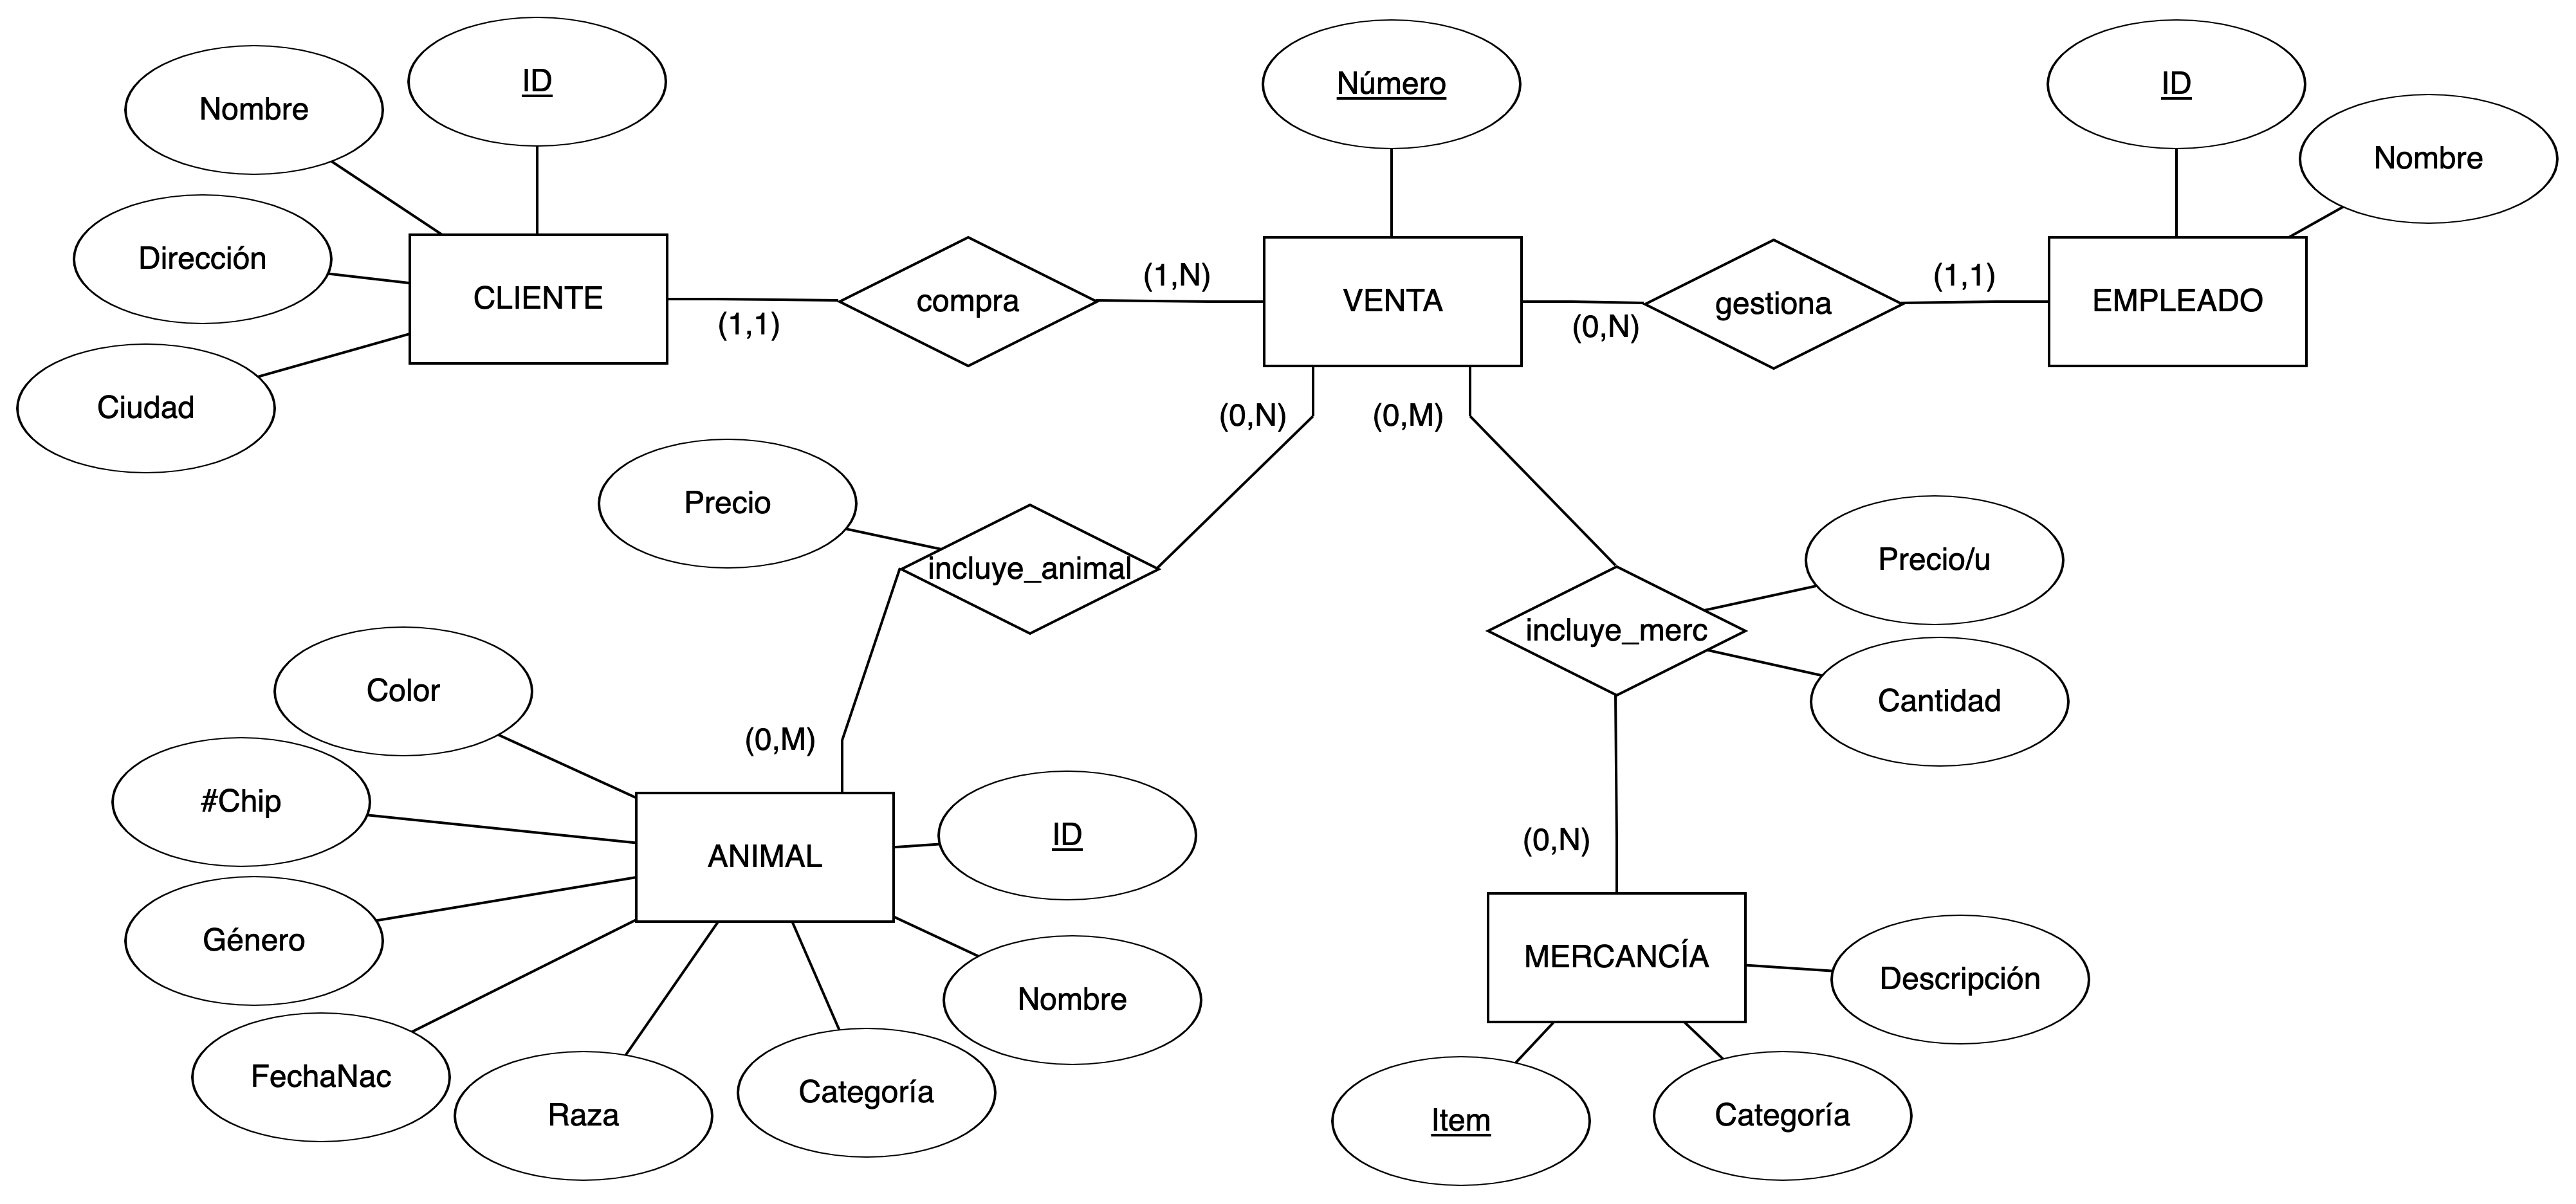
\includegraphics[width=\textwidth]{figs/tienda-de-mascotas}
\end{figure}

\newpage
\section{Permisos de circulación}

Transforme el siguiente modelo Entidad-Relación en un modelo relacional mediante las reglas del ``\textit{paso a tablas}'':

\begin{figure}[H]
    \centering
    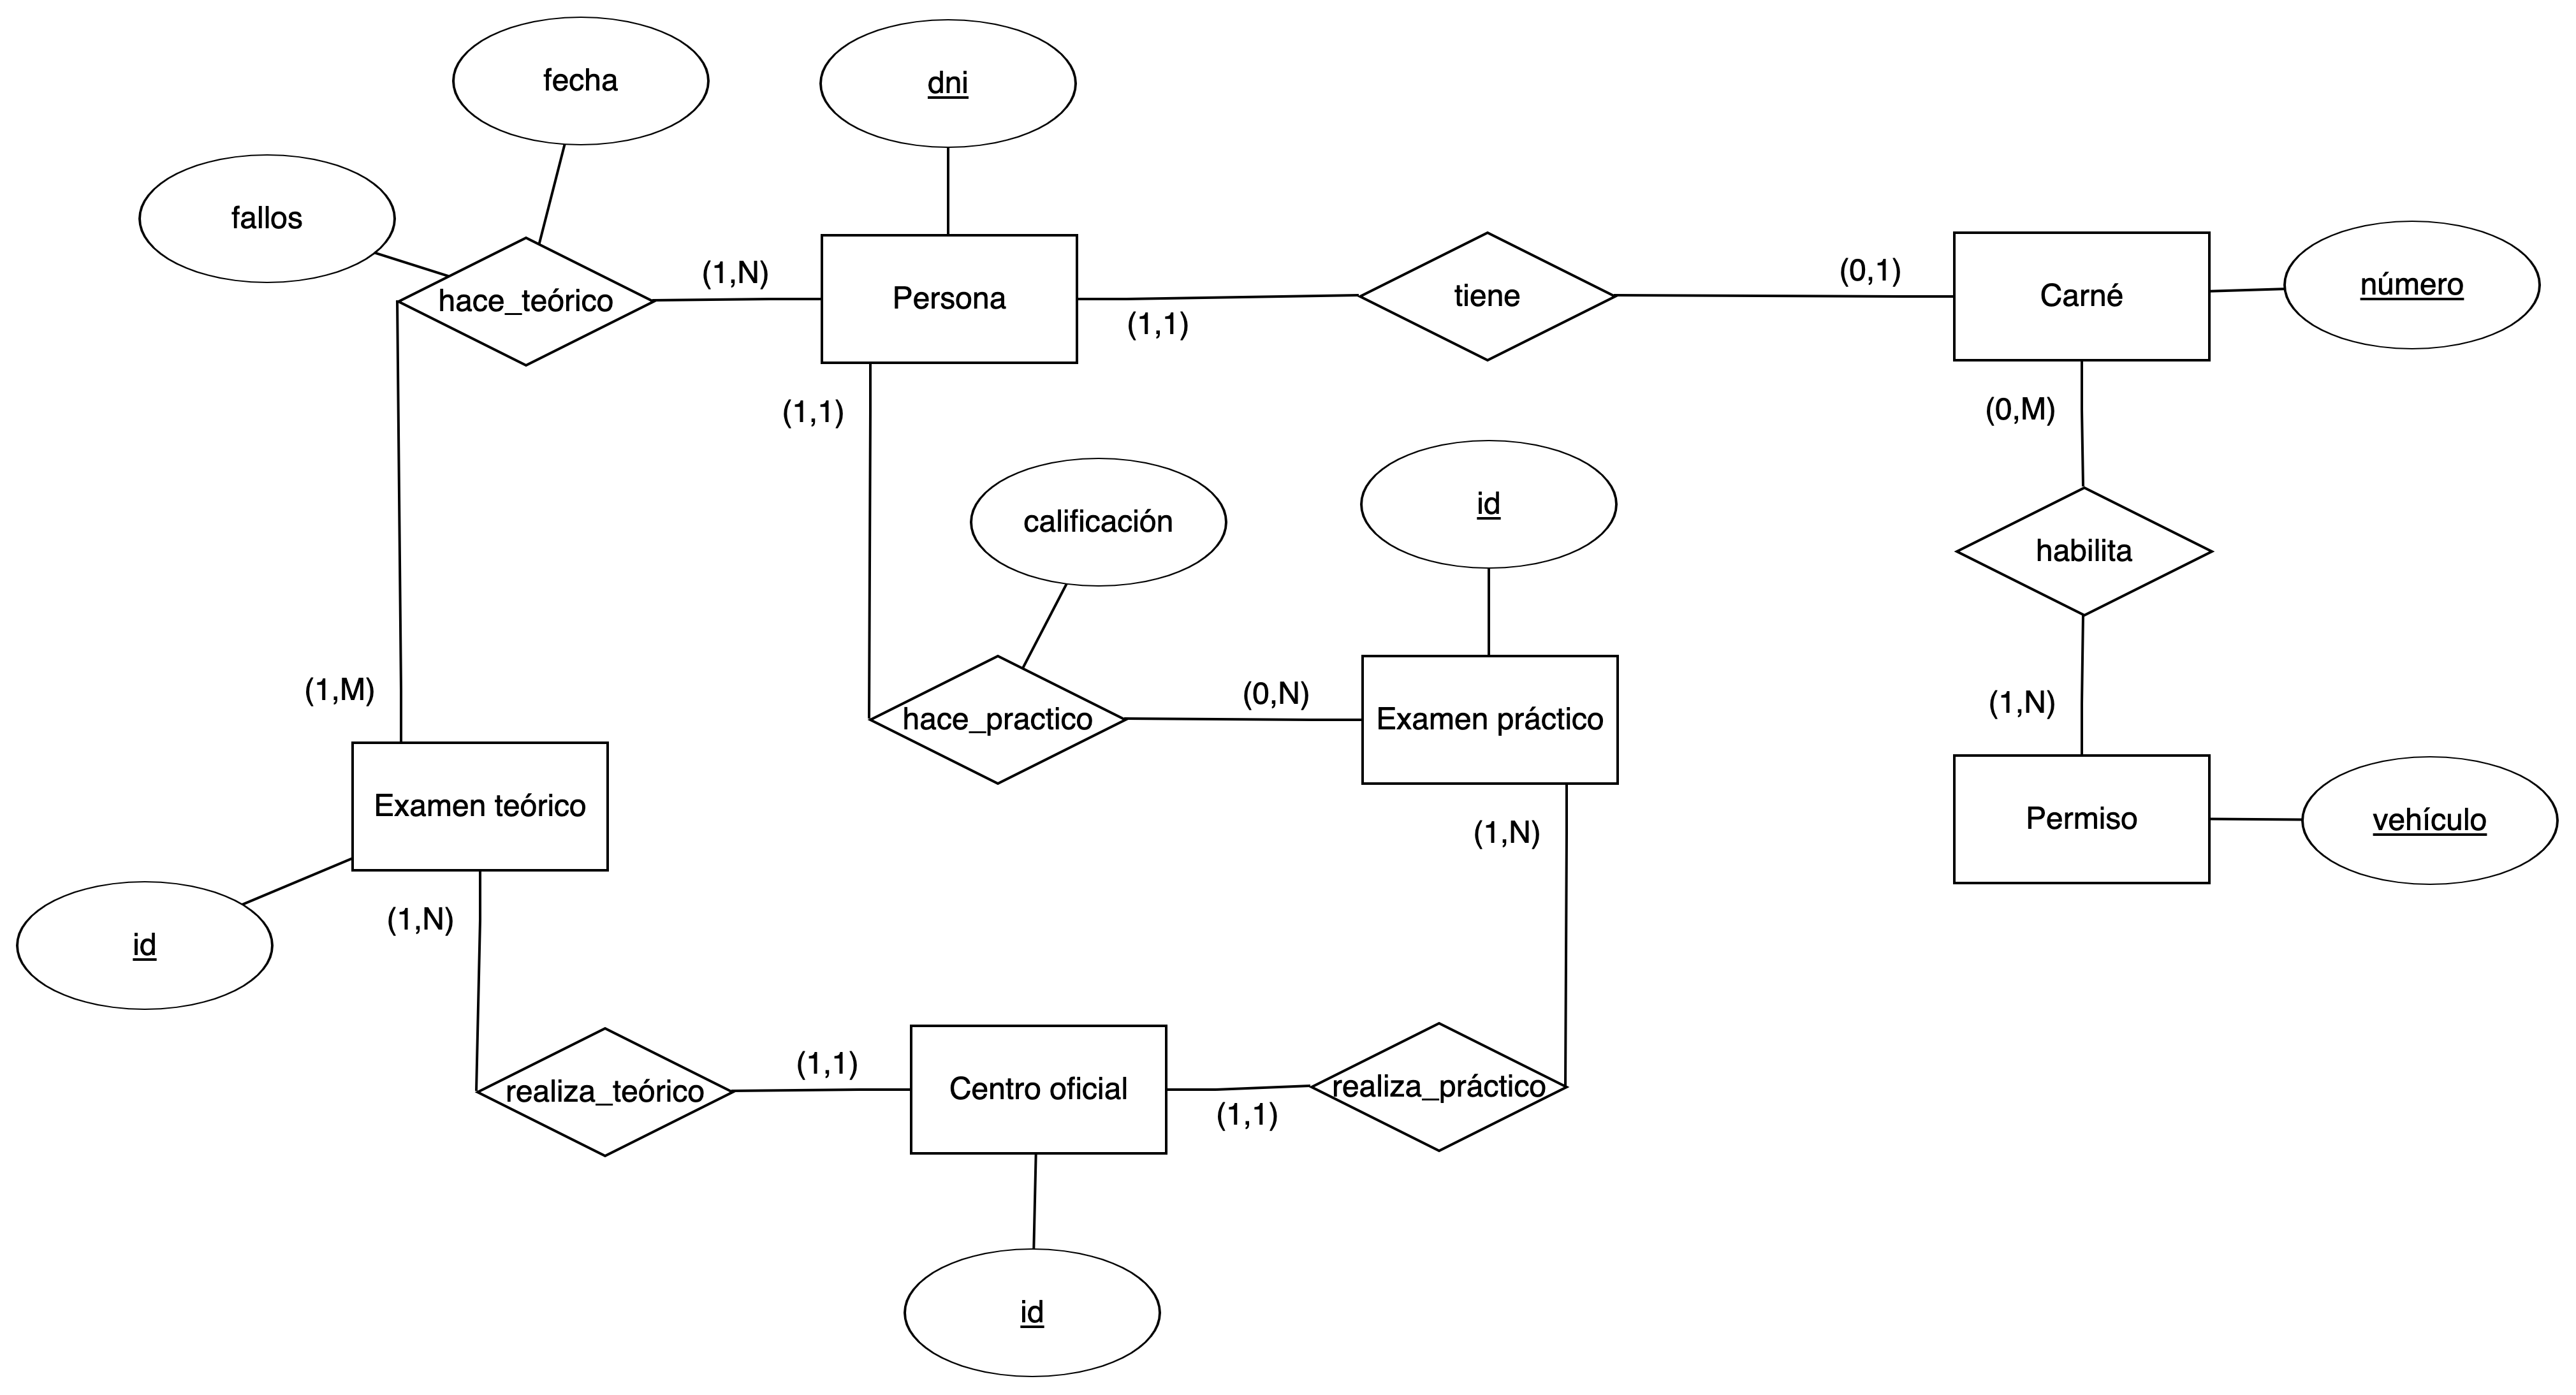
\includegraphics[width=\textwidth]{figs/permiso-de-circulacion}
\end{figure}

\section{Censo de la Unión Europea}

Transforme el siguiente modelo Entidad-Relación en un modelo relacional mediante las reglas del ``\textit{paso a tablas}'':

\begin{figure}[H]
    \centering
    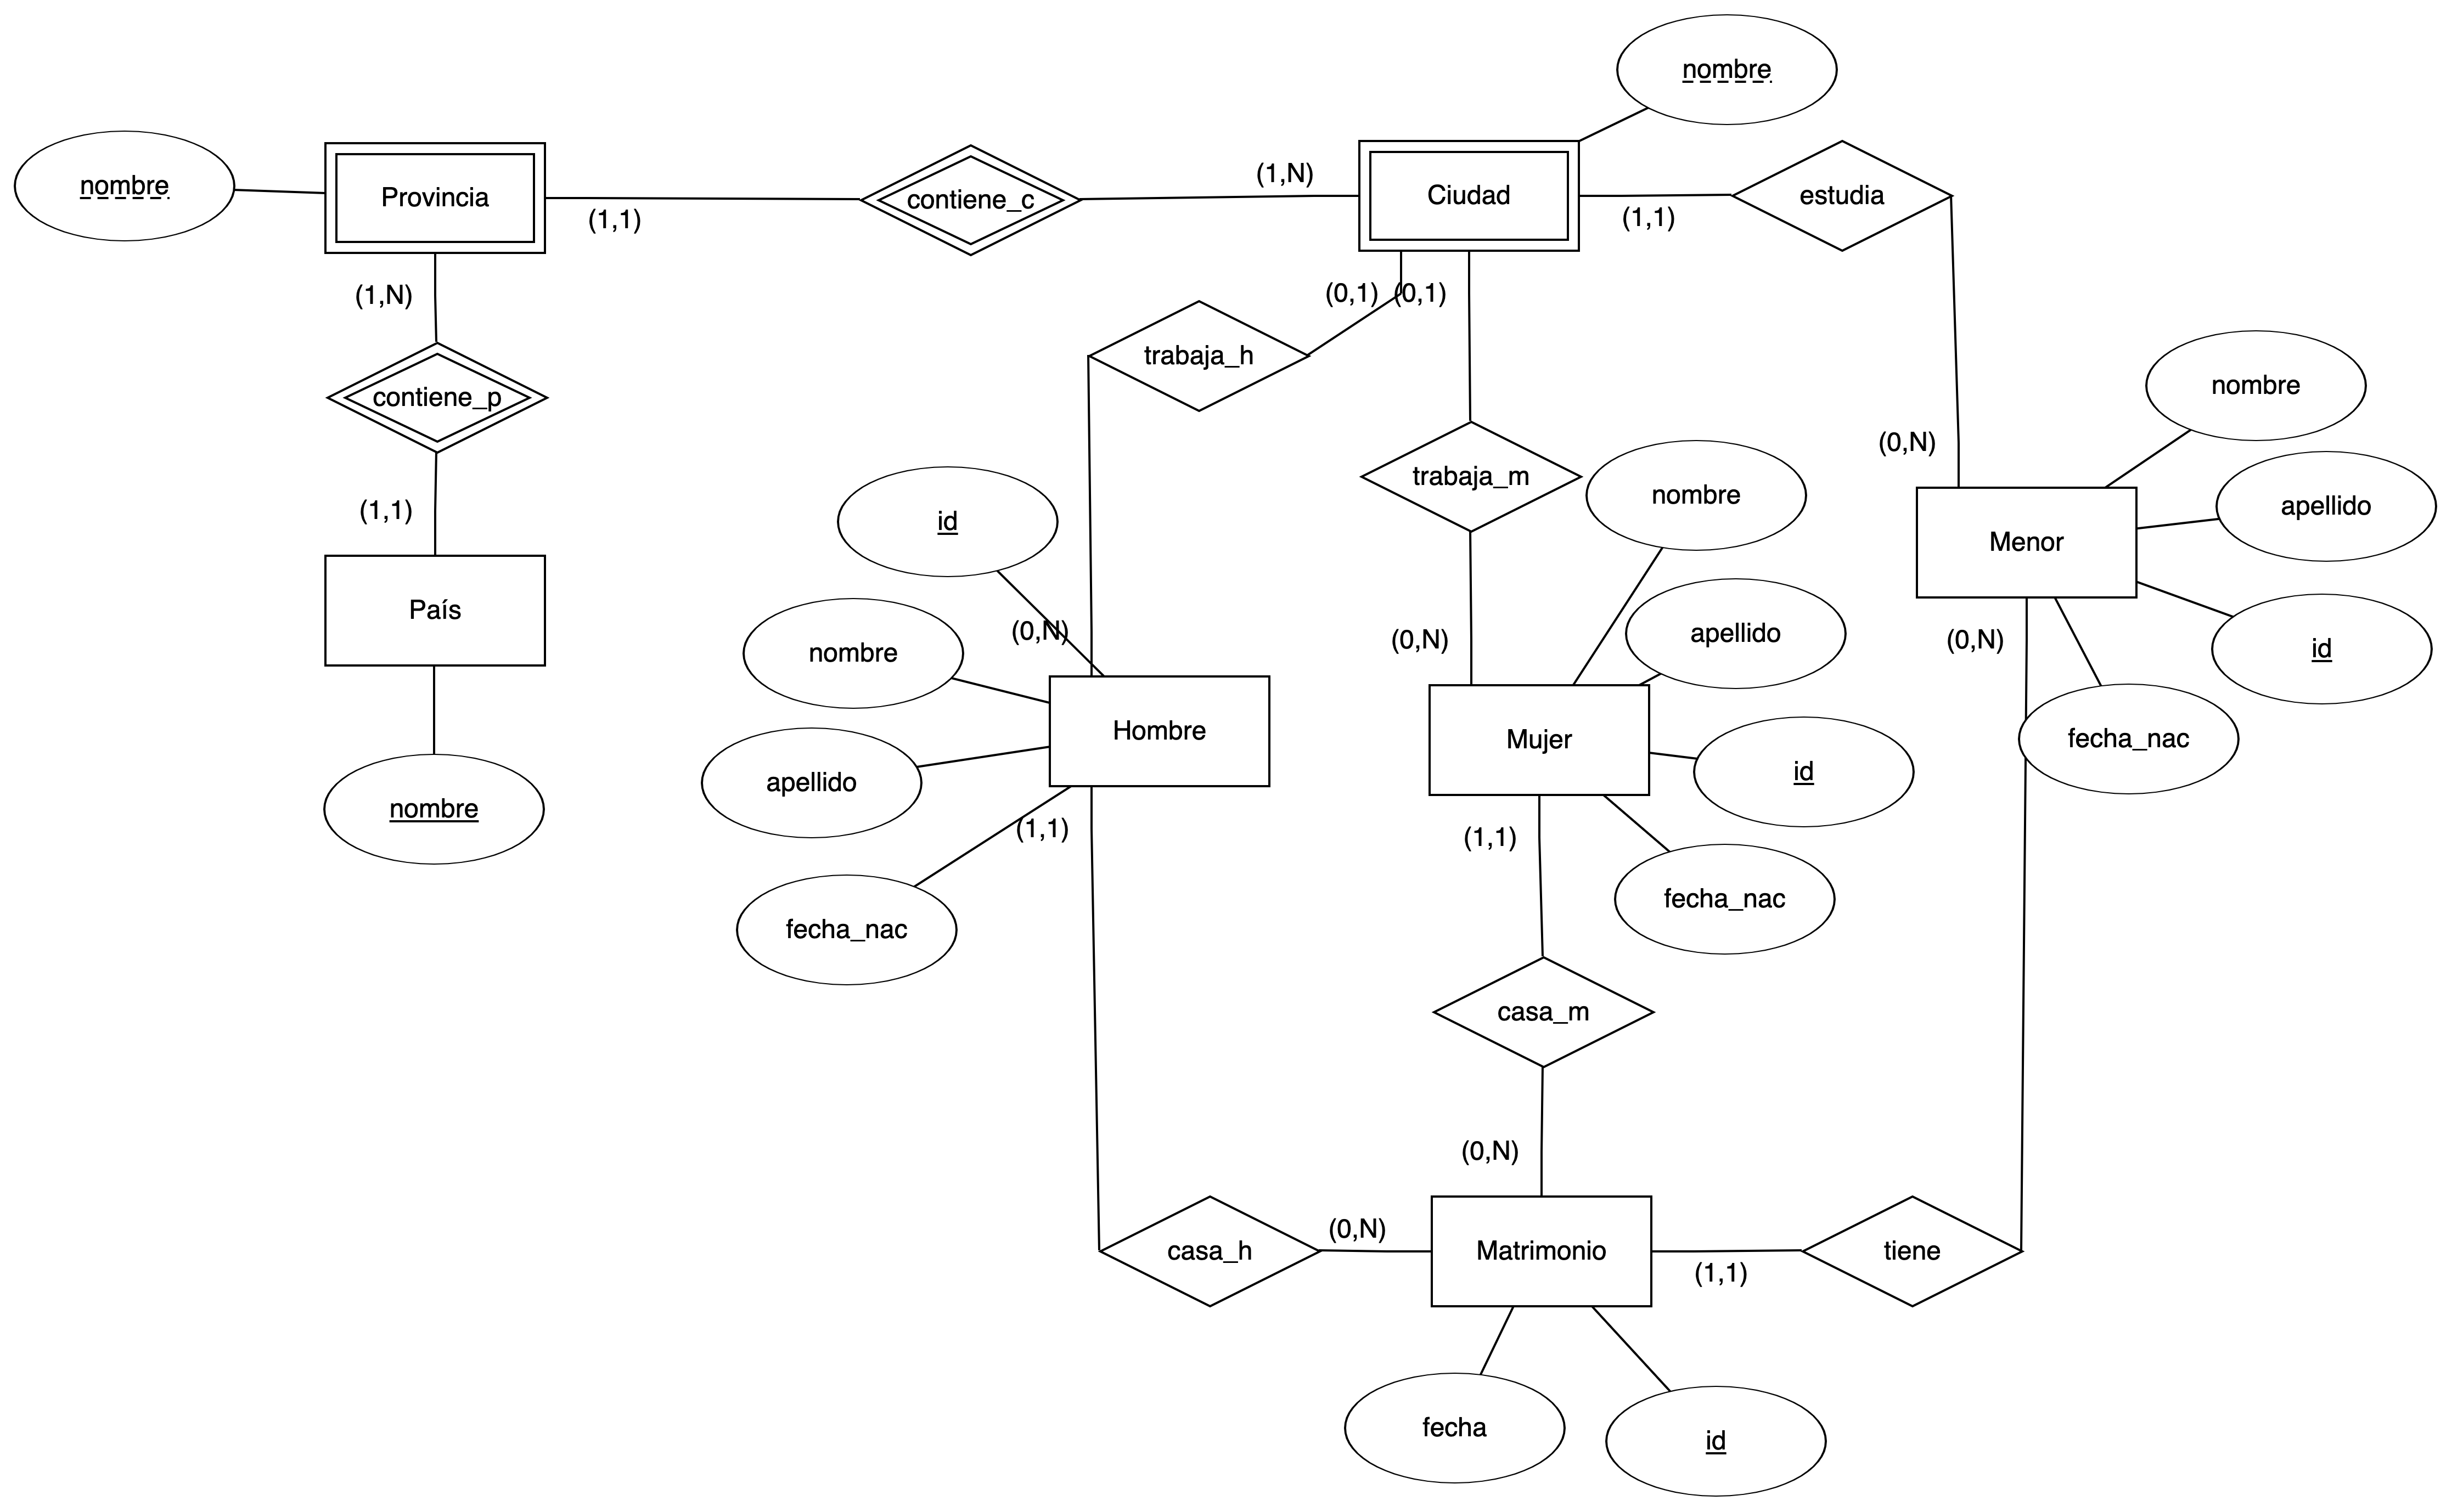
\includegraphics[width=\textwidth]{figs/censo-union-europea}
\end{figure}

\section{Desarrollo dirigidos por modelos}

Transforme el siguiente modelo Entidad-Relación en un modelo relacional mediante las reglas del ``\textit{paso a tablas}'':

\begin{figure}[H]
    \centering
    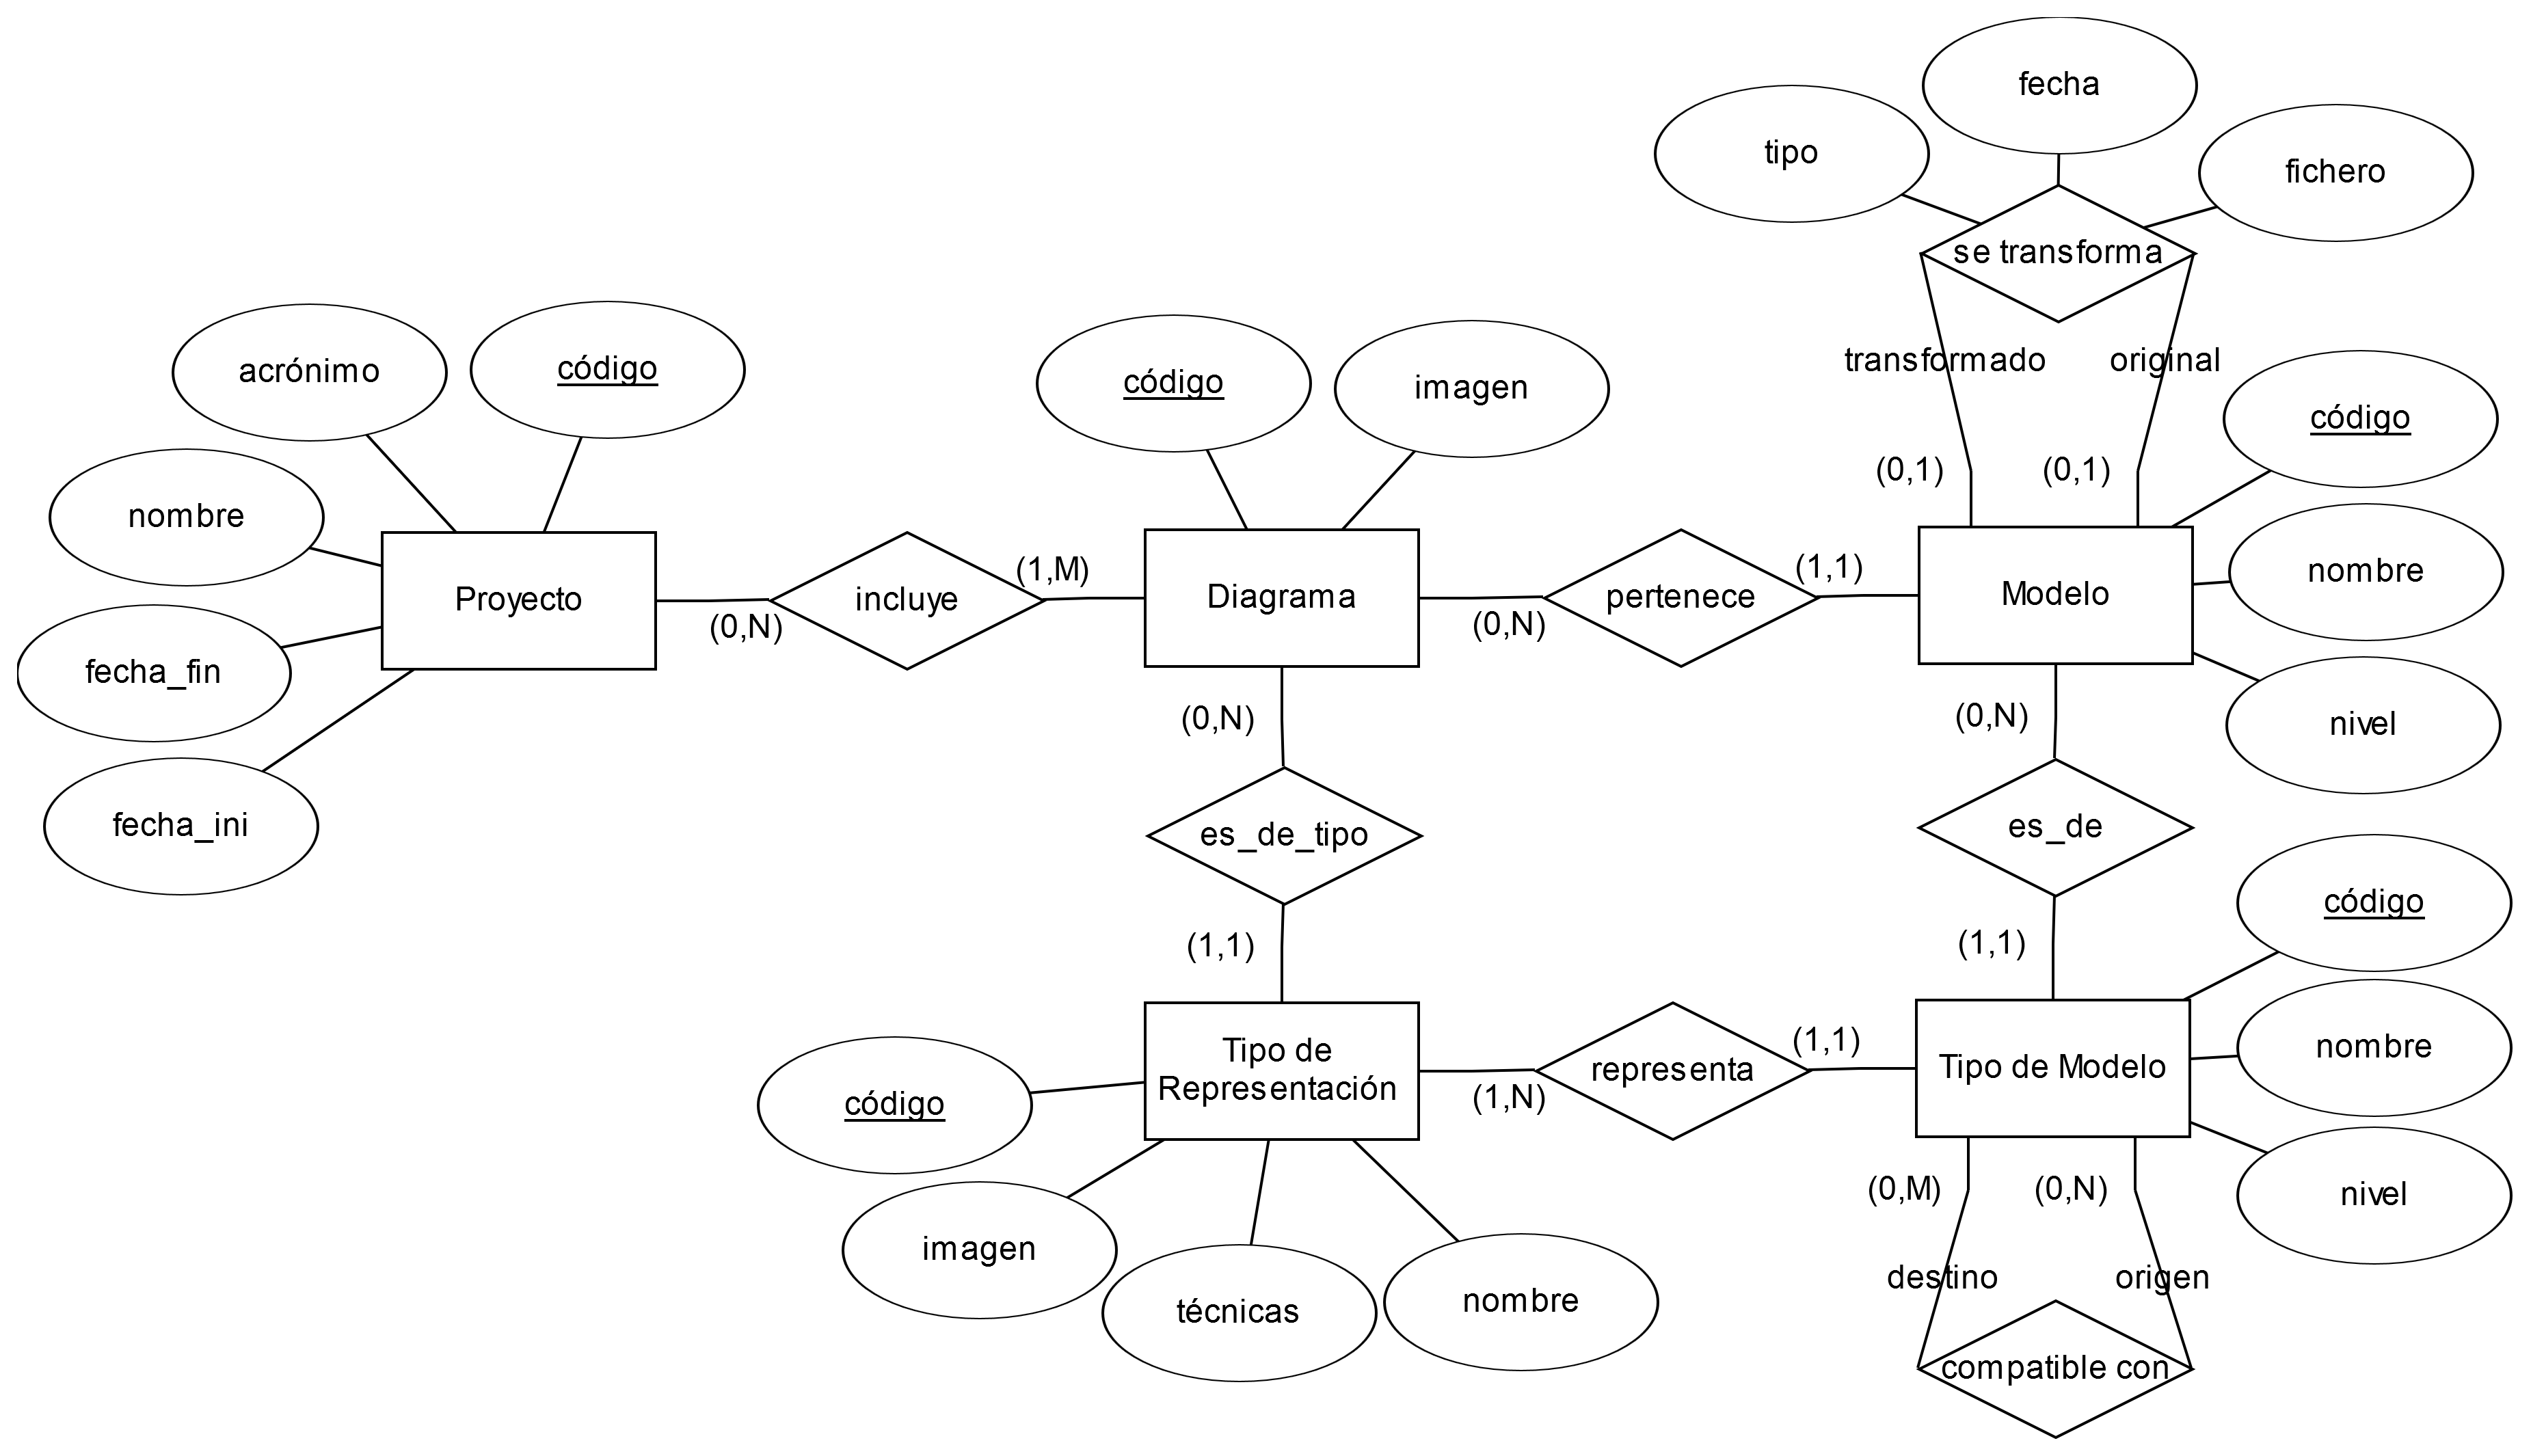
\includegraphics[width=\textwidth]{figs/desarrollo-dirigido-por-modelos}
\end{figure}

\section{Gestión de locales nocturnos}

Transforme el siguiente modelo Entidad-Relación en un modelo relacional mediante las reglas del ``\textit{paso a tablas}'':

\begin{figure}[H]
    \centering
    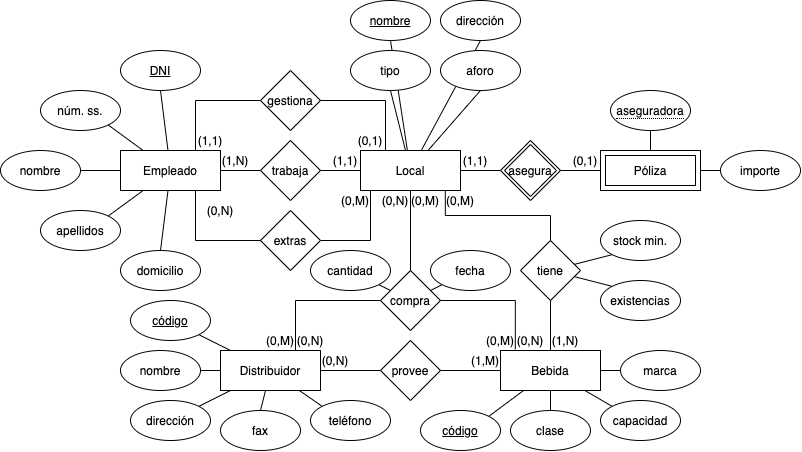
\includegraphics[width=\textwidth]{figs/gestion-locales-nocturnos}
\end{figure}

\newpage
\vspace{2em}
\hrule
\doclicenseThis

\end{document}
